% !TeX spellcheck = en_GB
\section{Evaluation}
\subsection{Calibration}
\subsubsection{Laser Power}
To set the power of the laser to a reasonable value a calibration curve was recorded which shows the actual laser power at the position of the microstrip plotted over the output power set in the GUI. This curve is shown in figure \ref{fig:power}.\\

Using this graph the output power was set to $P_\text{out}=20\,\mathrm{mW}$ which corresponds to an actual laser power of $P_\text{act}=(27.4\pm1.4)\,\mathrm{mW}$.
\begin{figure}[hb]
	\centering
	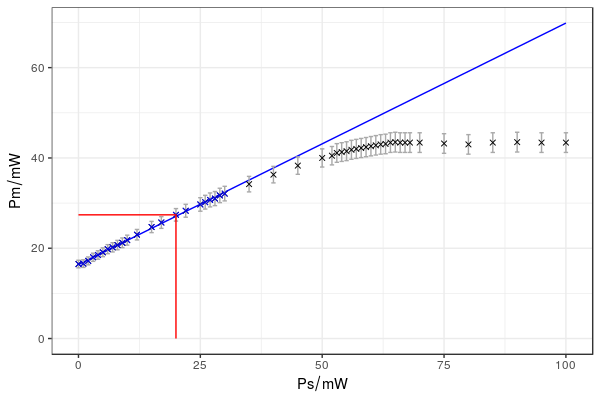
\includegraphics[width=\textwidth]{../figures/powercal.png}
	\caption{Measurement of the laser power}
	\label{fig:power}
\end{figure}

\subsubsection{Optical Spectrometer}
The optical spectrometer is later used to record the fluorescence spectrum of the diamond. To calibrate the optical spectrometer we first record the spectrum of visible light and compare the identified Fraunhofer lines with their literature values. The recorded spectrum is shown in figure \ref{fig:sunspectrum} and the values are given in table \ref{tab:fraunhofer}.\\

Since only small statistical deviations in both directions could be found there was no need to calculate a conversion factor and the values given from the optical spectrometer were verified. \\

The optical spectrometer was also used to get the actual wavelength of the laser which was determined in figure \ref{fig:laserspectrum} to be $\lambda=(517.3\pm0.2)\,\mathrm{nm}$.
\begin{figure}
	\centering
	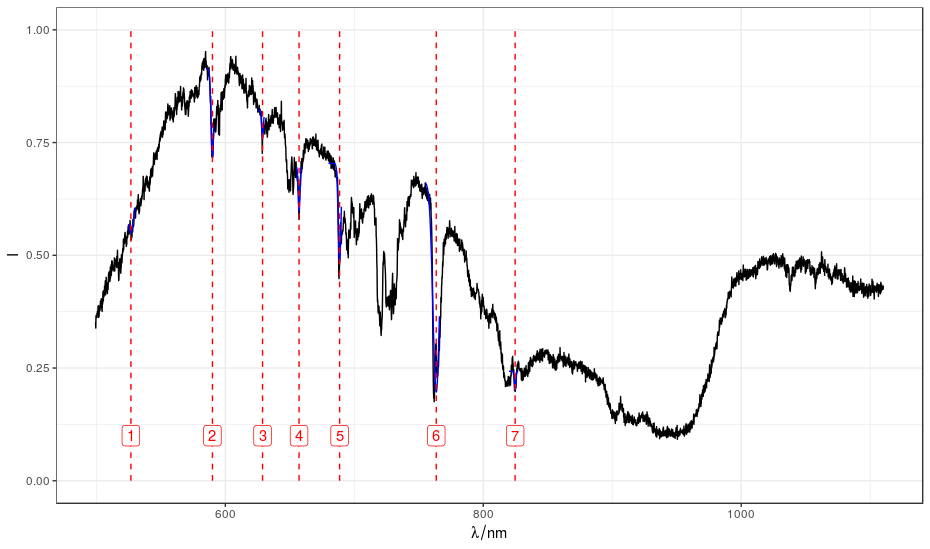
\includegraphics[width=0.8\textwidth]{../figures/sunspectrum.png}
	\caption[Spectrum of the sun with identified Fraunhofer lines]{Spectrum of the sun with identified Fraunhofer lines for calibration of the optical spectrometer}
	\label{fig:sunspectrum}
\end{figure}

\begin{table}
	\centering
	\begin{tabular}{c|c|c|c|c}
		Peak&Position&Element&Position \cite{fraunhoferlines}&Difference\\
		1&$526.8\pm1.7$&Fe I&527.0&$-0.2$\\
		2&$590.0\pm0.5$&Na I&589.6&$+0.4$\\
		3&$628.9\pm0.3$&Fe I&630.3&$-1.4$\\
		4&$657.2\pm0.3$&H $\alpha$&656.3&$+0.9$\\
		5&$688.6\pm0.5$&&&\\
		6&$763.5\pm1.3$&&&\\
		7&$824.7\pm0.3$&&&\\
	\end{tabular}
	\caption{Positions of the Fraunhofer Lines compared to the literature values}
	\label{tab:fraunhofer}
\end{table}

\begin{figure}
	\centering
	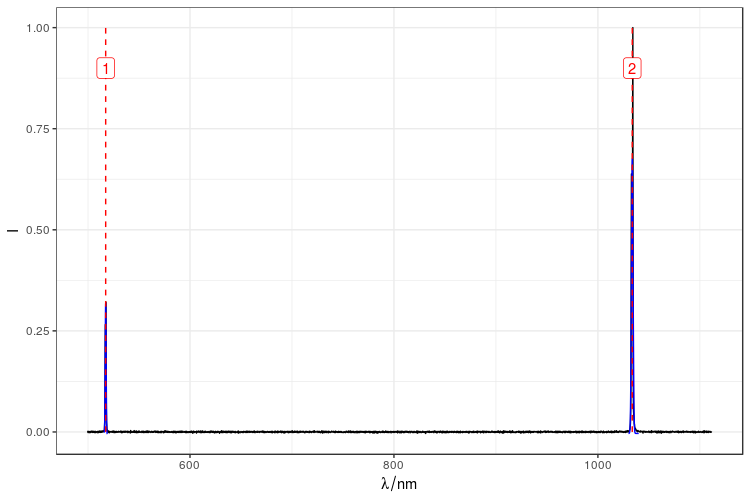
\includegraphics[width=0.8\textwidth]{../figures/laserspectrum.png}
	\caption[Spectrum of the laser]{Spectrum of the laser with identified peaks at the wavelengths $\lambda=(517.3\pm0.2)\,\mathrm{nm}$ and $\lambda=(1033.7\pm0.4)\,\mathrm{nm}$}
	\label{fig:laserspectrum}
\end{figure}

\subsubsection{ODMR calibrations}
\paragraph{Shielding}
To improve the ODMR signal and avoid noise generated by the microwaves a shielding cage was built around the APD. In figure \ref{fig:odmr-shield} the effect of this shielding cage on the ODMR spectrum is shown.
\begin{figure}
	\begin{subfigure}{0.5\textwidth}
		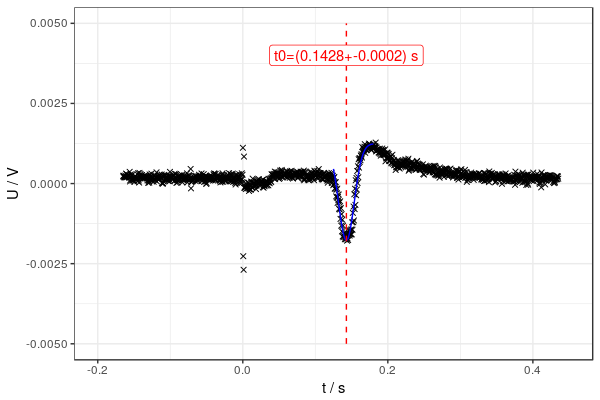
\includegraphics[width=\textwidth]{../figures/odmr-cal-1.png}
		\subcaption{without shielding}
	\end{subfigure}
		\begin{subfigure}{0.5\textwidth}	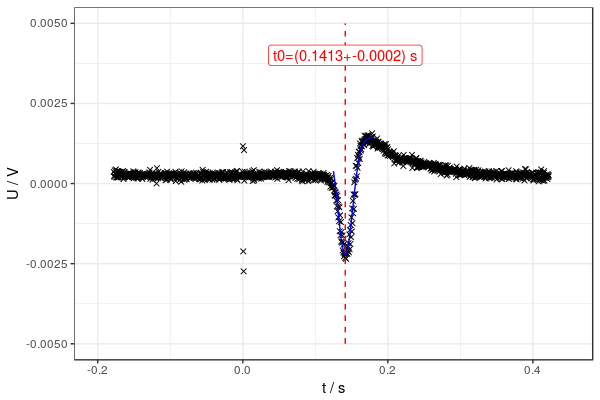
\includegraphics[width=\textwidth]{../figures/odmr-cal-2.png}
		\subcaption{with shielding}
	\end{subfigure}
	\caption{ODMR spectrum}
	\label{fig:odmr-shield}
\end{figure}
\paragraph{Time-to-Frequency Conversion}

\begin{figure}
	\begin{subfigure}{0.5\textwidth}
		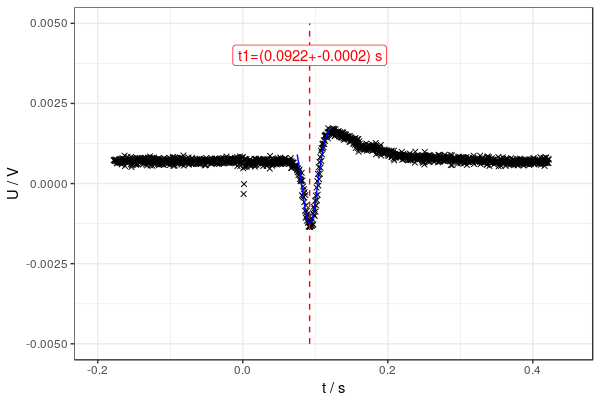
\includegraphics[width=\textwidth]{../figures/odmr-cal-4.png}
		\subcaption{shifted to the left}
	\end{subfigure}
	\begin{subfigure}{0.5\textwidth}
		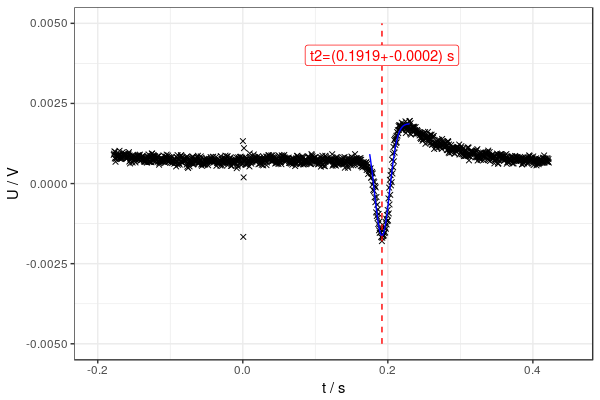
\includegraphics[width=\textwidth]{../figures/odmr-cal-3.png}
		\subcaption{shifted to the right}
	\end{subfigure}
	\caption{ODMR spectrum for time-to-frequency calibration}
	\label{fig:odmr-shift}
\end{figure}

Performing ODMR measurements we achieve the ODMR spectra on the oscilloscope. Therefore the spectra are time-resolved. To gain frequency-resolved spectra we need to calculate the conversion factor from time to frequency. We do this by performing two sweeps with shifted centre frequencies which allows us to calculate the conversion factor and also the offset since we know the frequency at which the peak appears.

The conversion can be expressed by the following equation:

\begin{align}
	f(t)&=\frac{f(t_1)(t_1-t_2)-(f(t_1)-f(t_2))t_1}{t_1-t_2}+\frac{f(t_1)-f(t_2)}{t_1-t_2}\cdot t
\end{align}

Inserting the values achieved from figure \ref{fig:odmr-shift} we get the following conversion function:

\begin{align}
	f(t)&=(1.003\pm0.003)\,\mathrm{\frac{GHz}{s}}\cdot t+(2.708\pm0.011)\,\mathrm{GHz}
\end{align}

Later in this document all spectra are converted by this function and therefore shown in the frequency domain. The errors are gained from the fit and propagated using Gaussian error propagation.

\subsection{Size of the Diamonds}

\subsection{Fluorescence Spectrum}
As indicated in section \ref{sec:nvcentres} the NV-centres exist in a NV$^-$ and a NV$^0$ state. While the ODMR-measurements can only be done on the NV$^-$ state we need to make sure that the diamond we found has NV$^-$ centres inside.\\

Therefore the fluorescence spectrum of the diamond is recorded and the position of the ZPL is determined. In figure \ref{fig:fluorescence} we see the ZPL to be at the position $\lambda_\text{ZPL}=(645\pm3)\,\mathrm{nm}$ which corresponds to an energy of $E_\text{ZPL}=(1.922\pm0.009)\,\mathrm{eV}$. This corresponds roughly to the energy given in figure \ref{fig:nvcentres}. So we verified the existence of NV$^-$ centres in the found diamond.
\begin{figure}
	\centering
	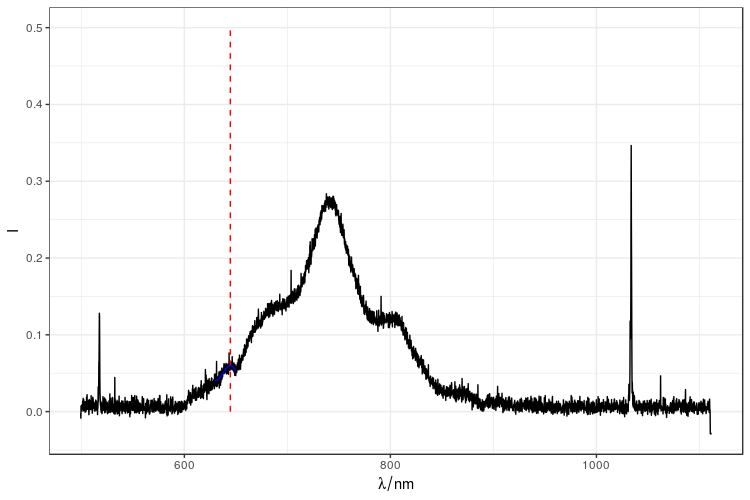
\includegraphics[width=0.8\textwidth]{../figures/fluorescence.png}
	\caption[Fluorescence spectrum of the diamond]{Fluorescence spectrum of the diamond with the zero phonon line (red line) at $\lambda_\text{ZPL}=(645\pm3)\,\mathrm{nm}$. The spectrum was achieved by averaging over 10 measurements.}
	\label{fig:fluorescence}
\end{figure}

\subsection{ODMR Measurements}
\begin{figure}
	\centering
	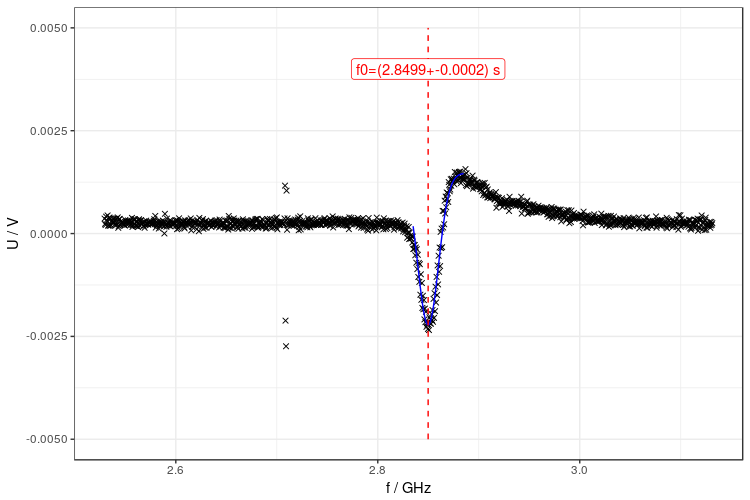
\includegraphics[width=0.8\textwidth]{../figures/odmr-1.png}
	\caption{ODMR Measurement of the diamond without a magnetic Field}
	\label{fig:odmr-no-B}
\end{figure}


\begin{figure}
	%\centering
	\begin{subfigure}{0.5\textwidth}
		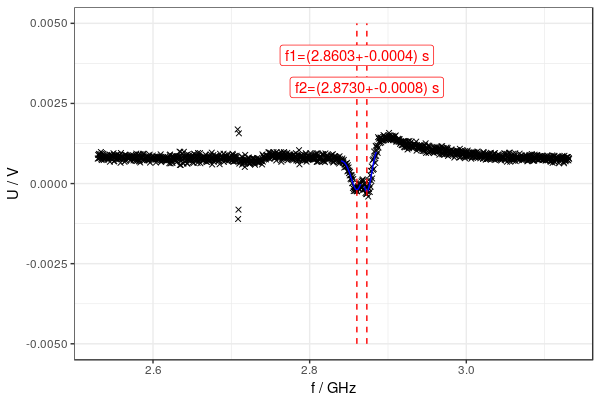
\includegraphics[width=\textwidth]{../figures/odmr-bx.png}
		\subcaption{Magnetic field in $x$-Direction}
	\end{subfigure}
	\begin{subfigure}{0.5\textwidth}
		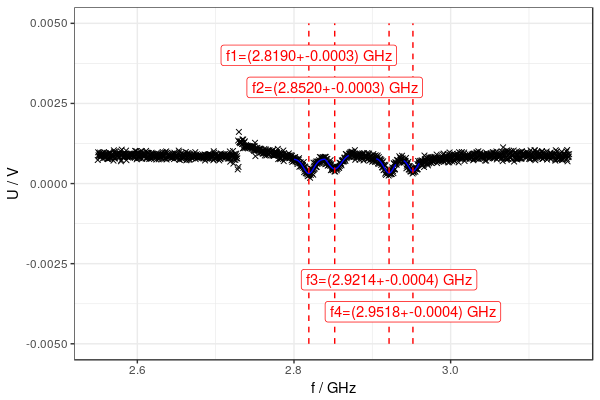
\includegraphics[width=\textwidth]{../figures/odmr-by.png}
		\subcaption{Magnetic field in $y$-Direction}
	\end{subfigure}
	\begin{subfigure}{0.5\textwidth}
		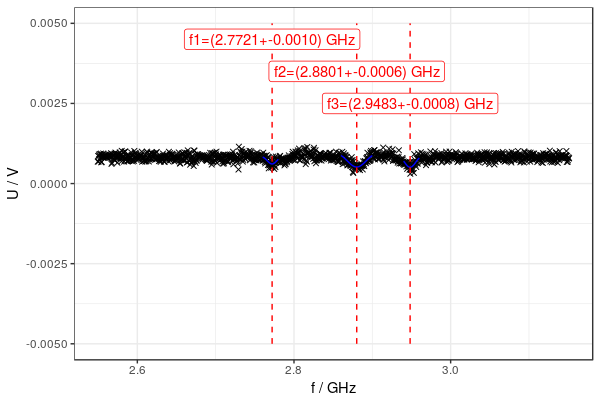
\includegraphics[width=\textwidth]{../figures/odmr-bz.png}
		\subcaption{Magnetic field in $z$-Direction}
	\end{subfigure}
	\caption{ODMR spectrum within a magnetic field}
	\label{fig:odmr-magnet}
\end{figure}

\begin{table}
	\centering
	\begin{tabular}{c|c|c}
		&Resonance 1&Resonance 2\\\hline
		$f_x / \mathrm{MHz}$&$6.2\pm0.5$&-\\
		$f_y / \mathrm{MHz}$&$34.7\pm0.4$&$66.5\pm0.4$\\\hline
		$B_x / \mathrm{mT}$&$0.214\pm0.018$&-\\
		$B_y / \mathrm{mT}$&$1.197\pm0.014$&$2.297\pm0.014$\\\hline
		$d_x/d$&$0.036\pm0.003$&-\\
		$d_y/d$&$0.203\pm0.002$&$0.389\pm0.002$
	\end{tabular}
	\caption{Resonance Pairs}
\end{table}